% 1.3.Cmake.tex
%	Last update: 2020/02/27 F.Kanehori
%\newpage
\subsection{cmake}
\label{subsec:CmakeLibrary}
\parindent=0pt

以下では、CMakeの生成物(ビルドの生成物ではありません)を格納する
作業場所(ディレクトリ)を\DQuote{\BldDir}として話を進めます
(作業場所の名前は任意で構いません)。

\medskip
CMakeにはConfigureとGenerateの2段階があります。

\medskip
コマンドプロンプトの場合は、1回のコマンドで両方を実行できます。
\Vskip{-.5\baselineskip}

\CmndLine{%
	> chdir C:/Springhead\\
	> mkdir build\\
	> cmake -B build [\it{generator}]
}{command-1-3.eps}{cmake}

\medskip
\it{generatorの}詳細は、コマンドプロンプトで\tt{cmake --help}とすると確認できます。

\it{generator}を省略した場合のデフォルトは、
Windowsの場合にはインストールされているVisual Studioの最新バージョンが、
unixの場合には\tt{Unix Makefiles}が選択されるようです。
ただし、マシンアーキテクチャは自動的には判定されません。
Windowsで64ビットマシンの場合には \tt{-A x64}を指定してください。

\begin{narrow}[s]
	\Vskip{-.2\baselineskip}\thinrule{\linewidth}\\
	\it{generator}の例\\
	\begin{tabular}{@{\hspace{5pt}}l@{\hspace{10pt}}l}
	    Windows:	& \tt{-G "Visual Studio 15 2017" -A x64} \\
	    unix:	& \tt{-G "Unix Makefiles"} \\
	\end{tabular}\\
	\Vskip{-.2\baselineskip}\thinrule{\linewidth}\\
\end{narrow}

\Vskip{-.5\baselineskip}
cmake--guiを利用する場合は、
まず、次の画面でConfigureボタンを押します。
\begin{narrow}[15pt]
	\begin{figure}[h]
	\begin{center}
	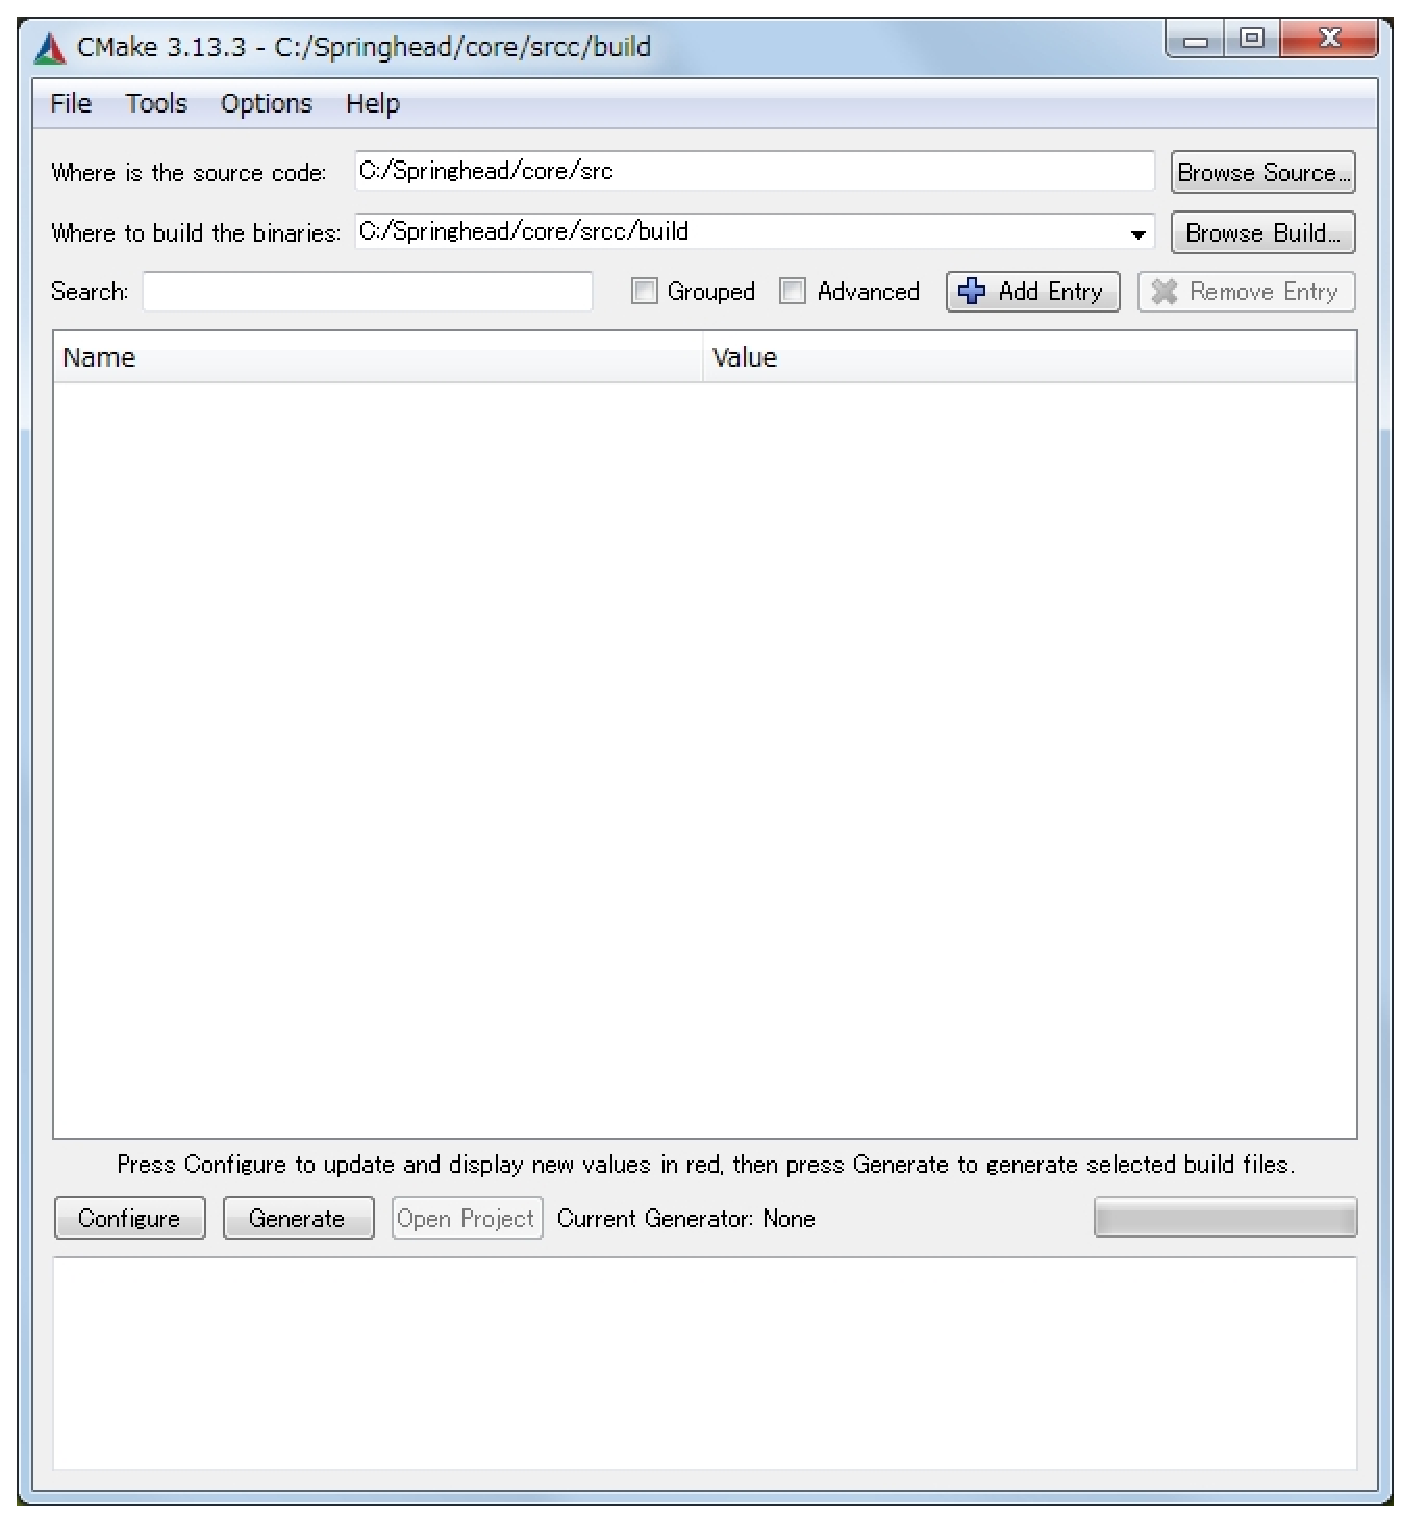
\includegraphics[width=0.7\textwidth]{fig/CmakeConfigure1.eps}
	\end{center}
	\caption{\cmake\ configure}
	\label{fig:CmakeConfigure}
	\end{figure}
\end{narrow}

\DQuote{\BldDir}ディレクトリがなければ作成するかどうかを尋ねられ、
\begin{narrow}[15pt]
	\begin{figure}[h]
	\begin{center}
	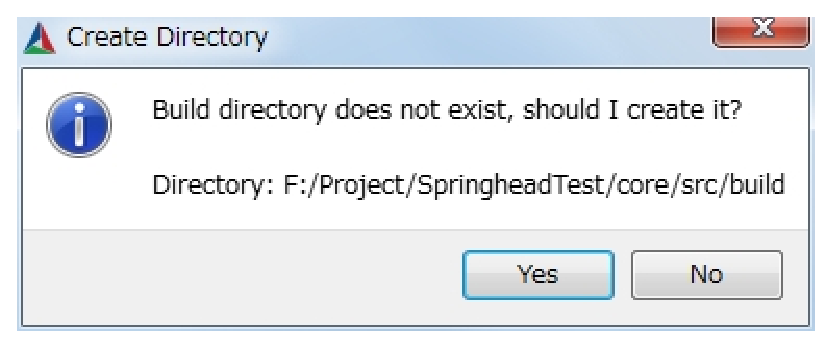
\includegraphics[width=0.5\textwidth]{fig/CmakeConfigure2.eps}
	\end{center}
	\caption{\cmake\ configure}
	\label{fig:CreateWorkSpace}
	\end{figure}
\end{narrow}

次にgenerator指定画面となります。
\begin{narrow}[15pt]
	\begin{figure}[h]
	\begin{center}
	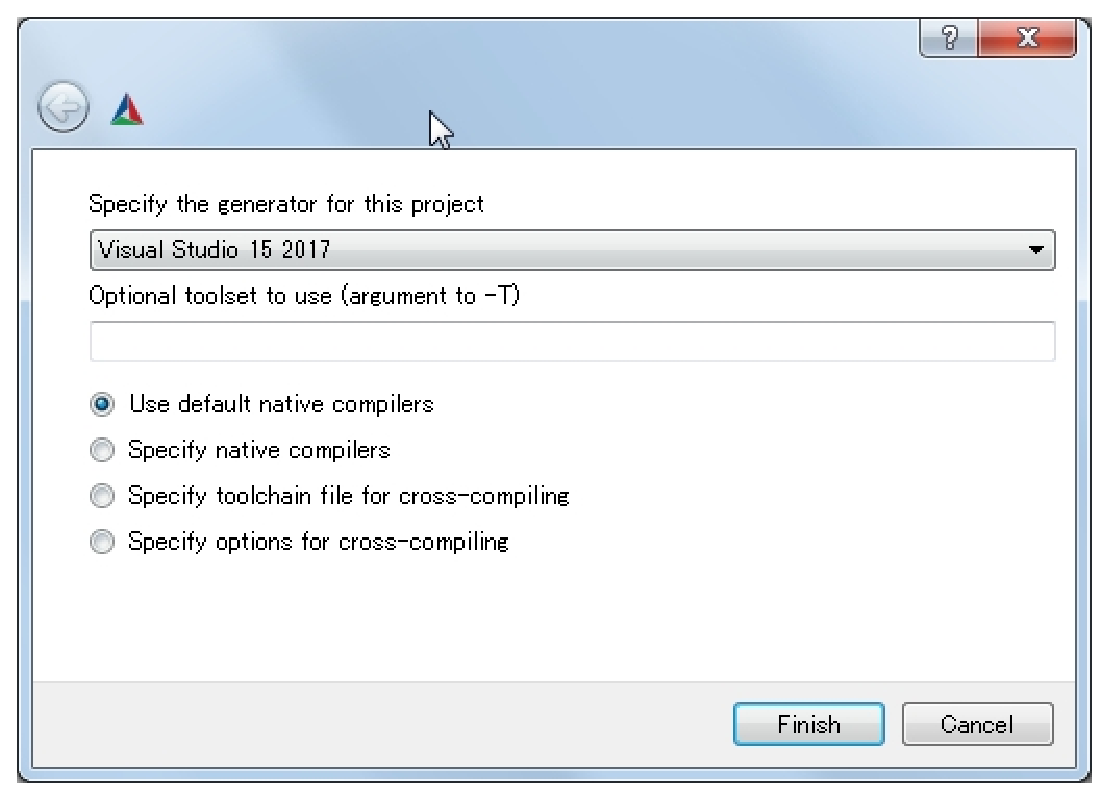
\includegraphics[width=0.6\textwidth]{fig/CmakeConfigure3.eps}
	\end{center}
	\caption{\cmake\ configure}
	\label{fig:CmakeGeneration}
	\end{figure}
\end{narrow}

最後に図\ref{fig:CmakeConfigure} のGenerateボタンを押します。

\medskip
以上で、\DQuote{\BldDir}以下にsolution file / project file (Windowsの場合)
またはMakefile (unixの場合)などが生成されたはずです。

% end: 1.3.Cmake.tex
